\section{Background}
We begin with related background on \nn-based video analytics, and 
then present the space \nn configurations that affects the balance
between accuracy and resource consumption.

\subsection{Video analytics}
%We begin with a high-level overview of the recent video analytics
%systems and their typical quality/performance requirements. 
%More importantly, we show that setting the key configurations 
%can strike a favorable balance between resource consumption and 
%accuracy.
Applications based on accurate video analytics are ubiquitous in our
daily life; e.g., tracking vehicle traffic, pedestrian, and accidents
has become de-facto components of road traffic management and 
self-driving cars.
In this paper, we focus on improving the performance of object 
detection, where the goal is to identify objects of interests (and
sometimes their locations) in each frame.
Object detection is a basic analytics task on which a wide range of 
higher-level tasks (e.g., vehicle collisions, speeding detection)
are built.

\mypara{Object detection on live video feeds}
As shown in Figure~\ref{fig:overall}, 
a video analytics system takes as input video feeds potentially from
many cameras, and a video analytics query from an analyst,
and returns the query output on the video feeds typically on a 
frame-by-frame basis.
In its simplest form, an object detection query specifies the classes 
of object of interest (e.g., vehicles), the video feed, and the 
time duration for which the task would continuously run. 
% From these basic queries, one can build higher-level queries,
% such as traffic accident detection by combining queries of vehicle
% tracking and pedestrian detection.
% In this paper, we focus on improving the performance of basic queries.
While object detection can be applied to any image, we focus on object 
detection in on live video feed. 
While \name is applicable to offline video, we pick live videos
for two reasons.
%\begin{packeditemize}
%\item 
First, because it is hard to predict when the objects of interest 
would appear in a live feed, live video queries are typically 
long-lasting (even indefinite).
% Because the content in a live video stream is hard to predict, queries
% over live videos often run for a long time to find objects 
% or events of interest. %\jc{some example of real world?}
%\item 
Second, live video analytics is very {\em resource-demanding}, as it
must process the video at the same speed as the frame encoding rate,
and such cost grows proportionally to more queries and video feeds.
%, i.e., one-second worth of video 
%must be processed within one second, otherwise the delay could 
%accumulate over time.
% For instance, running Yolo detector on a 30 frames/second video stream
% once requires a \$\fillme GPU. 
% Such cost does not share across queries or video feeds, and thus can 
%\end{packeditemize}
As we will see, both long duration and high resource consumption 
bear implications to the need for online profiling.

\mypara{Performance metrics}
The performance of object detection is measured by accuracy and 
resource consumption.
\begin{packeditemize}
\item {\em Accuracy:} 
Accuracy of an \nn inference output (a list of bounding boxes each 
with its location and object label) is defined by the F1 score between
these  objects and the ground truth (also in the form of a list of
labeled bounding boxes). 
Specifically, we use the method proposed in vision 
community~\cite{http://homepages.inf.ed.ac.uk/ckiw/postscript/ijcv_voc09.pdf}
to map the detected objects and the objects in the ground truth, 
and then calculate the F1 score, which includes both precision and 
recall.
\item {\em Resource consumption:}
We use average GPU processing time (under 100\% utilization) per frame
as the metric of resource consumption.
While running modern deep \nn models takes more resources than GPU 
cycles, GPU is much more expensive than other resources.
What's more, \nn requires more GPU cycles than any big data tasks while
their demands for other resources are on par.
% Specifically, we define the resource consumption as the amount of 
% resources needed by a \nn model to produce inference results on each 
% one second worth of video feed.
\end{packeditemize}

\subsection{Pipelines and the configuration space}

\mypara{Object detection pipelines}
A video analytics system runs an object detection query by feeding 
a sequence of frames to an \nn inference model.
We consider two inference pipelines as depicted in 
Figure~\ref{fig:pipeline}.
In pipeline $A$, the raw video frames are first preprocessed, 
which typically involves frame sampling and resizing, and the sampled,
resized frames are then fed to a pre-trained object-detection model
(e.g., Faster RCNN~\cite{??}, Yolo~\cite{??}). 
Pipeline $B$ uses a light-weight background subtraction logic (a 
non-\nn model for which CPU is sufficient) to crop out the region of 
interests from the frames, and sends only these smaller images to an
\nn-based classifier 
(e.g., ResNet~\cite{??}, MobileNet~\cite{??}) to get their labels.
Both pipelines have been actively studied in the computer vision 
literature.
While pipeline $A$ attracts more attention recently as it is more 
generic, pipeline $B$ bears the advantage of not having to process 
the whole frame, when the targeted objects rarely appear.

\mypara{Configuration space}
Each pipeline has several important configurations, or {\em knobs},
whose values are critical to the performance (accuracy and resource consumption) of
object detection. 
\begin{packeditemize}
\item 
In pipeline $A$, we consider three knobs: {\em frame rate}, 
{\em input image size}, and the pre-trained 
{\em object detection model}. 
That is, the frame rate and the input image size decide which 
frames and in what size should be fed to the object detection model.
\item 
In pipeline $B$, we consider two knobs: {\em minimal area
size}, and the pre-trained {\em classifier model}.
That is, only regions larger than the minimal area size will be 
sent to the classifiers for labeling.
\end{packeditemize}

Note that while most proposals in the literature are based on these
two pipelines with these tunable knobs, we notice there are other 
object detection pipelines~\cite{??} and more tunable knobs.
Optimizing for more pipelines is certainly an interesting future 
work, but it is beyond the scope of this paper. 


\subsection{Impact of configurations on performance}
Next, we will quantitatively show how these configurations affect
performance.


% \begin{figure}[h!]
% \centering
% 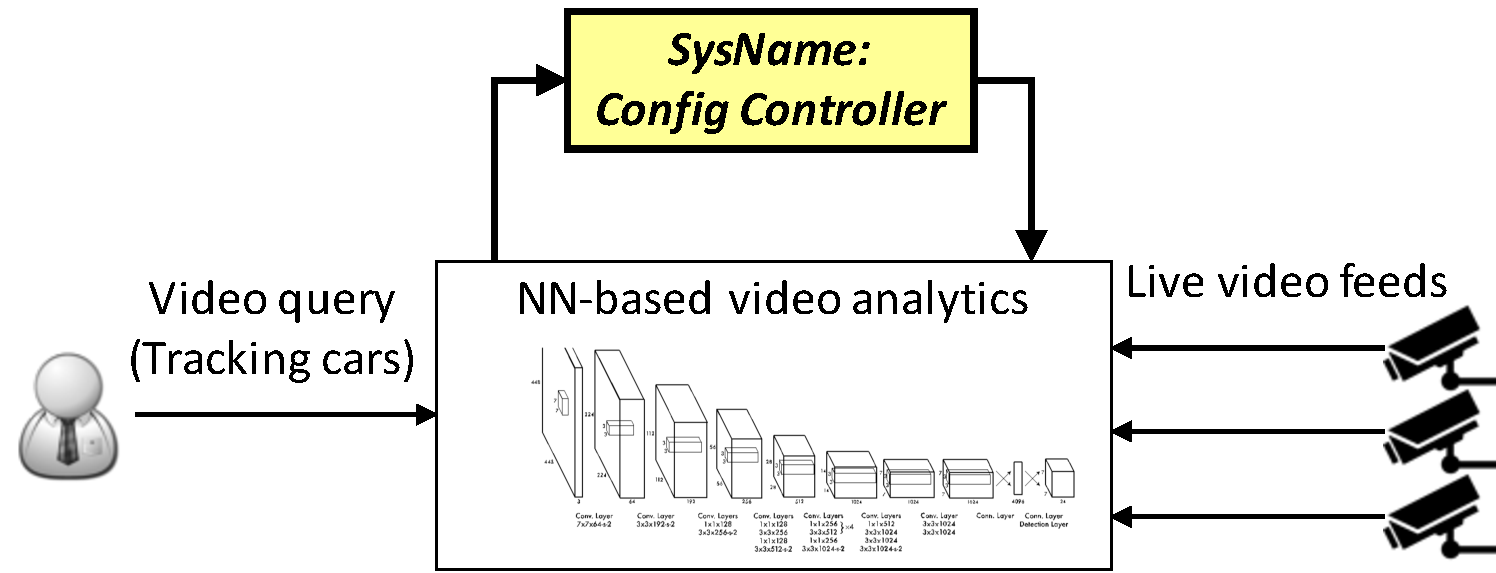
\includegraphics[width=0.4\textwidth]{figures/Overall.pdf}
% \vspace{-0.2cm}
% \tightcaption{Overview of \name, which features the configuration 
% controller that profiles the performance of different configurations
% and dynamically picks the best one.}
% \label{fig:overall}
% \end{figure}

%\mypara{Live video analytics}
While \nn can be applied to both live and offline videos, we focus on
optimizing {\em live video} analytics (the same techniques can be 
applied to offline video analytics too).
Live video analytics has two unique features.
%\begin{packeditemize}
%\item 
First, live video queries are {\em long-lasting}, sometimes without 
pre-determined end time; e.g., tracking cars captured by a traffic 
camera at a cross-road for a whole week.
Because the content in a live video stream is hard to predict, queries
over live videos often run for a long time to find objects 
or events of interest. %\jc{some example of real world?}
%\item 
Second, live video analytics is very {\em resource-demanding},
as it must process input videos in real-time speed.
%, i.e., one-second worth of video 
%must be processed within one second, otherwise the delay could 
%accumulate over time.
For instance, running Yolo detector on a 30 frames/second video stream
once requires a \$\fillme GPU. 
Such cost does not share across queries or video feeds, and thus can 
grows proportionally to more queries and video feeds.
%\end{packeditemize}
Both properties of long duration and high resource consumption bear
implications to the need for adaptive profiling, as we will see.

\mypara{Performance metrics}
The performance of a video analytics system is measured by two 
seemingly contradicting metrics:
\begin{packeditemize}
\item {\em Accuracy:} 
On one hand, we want the \nn inference results, in the form of a list
of bounding boxes indicating the location and label (e.g., a car) of 
each object, to be identical to the ground-truth locations of the 
objects.
Specifically, we use {\em mean average precision} (mAP)
\cite{http://homepages.inf.ed.ac.uk/ckiw/postscript/ijcv_voc09.pdf}
\footnote{While mAP is commonly used in the literature, we note that 
other metrics (e.g., F1 scores) are sometimes used, and we observe
similar results in F1 score too.}
to measure the accuracy.
\item {\em Resource consumption:}
On the other hand, we want to minimize the resource consumption such 
as GPU and CPU utilization and RAM size. 
Specifically, we define the resource consumption as the amount of 
resources needed by a \nn model to produce inference results on each 
one second worth of video feed.
\end{packeditemize}

\mypara{Configurations}
Several configurations of a video analytics can impact on its 
performance, either accuracy, resource consumption, or both.
They are two general categories of such configurations.
\begin{packeditemize}
\item {\em Video-specific configurations:}
Before the input video is fed to \nn, it can be adjusted in several 
ways, such as video resolution, frame rate, brightness, contrast, and
so forth.
\item {\em \nn-specific configurations:}
Given an input video, we can also pick \nn parameters, such
as confidence threshold (the \nn model only report the objects 
detected) and input resolution (the size the \nn treats an image 
internally), and choose among several pre-trained \nn models.
\end{packeditemize}


\subsection{The need for adapting configurations}

\subsubsection{Impact of configurations on \nn performance}
While maximizing accuracy and minimizing low resource consumption 
seems contradictive, prior work has shown that we could strike a 
favorable balance between accuracy and resource consumption by 
picking suitable values for key configurations of running 
\nn~\cite{videostorm,noscope}.
For instance, Figure~\ref{fig:example} shows the accuracy and 
resource consumption (in terms of GPU utilization) of using various 
frame rates on the same video clip. 
 You can see that while the highest accuracy is achieved at the 
highest frame rate (highest resource consumption), there is a 
sweet-spot where a near-optimal accuracy (e.g., \fillme) can be 
achieved by a \fillme\% lower frame rate.
\jc{maybe add graphs for other configs}


\subsubsection{Optimal configurations are dynamic}

Naturally, it is tempting to optimize video analytics performance by
profiling the resource-accuracy tradeoffs of various configurations
and picking the optimal configuration before each analytics query 
(which is what prior work does).
However, the optimal configurations have substantial temporal 
variability even for the same video feed. 
There are two sources behind this dynamics.


%\begin{figure}[h!]
%\centering
%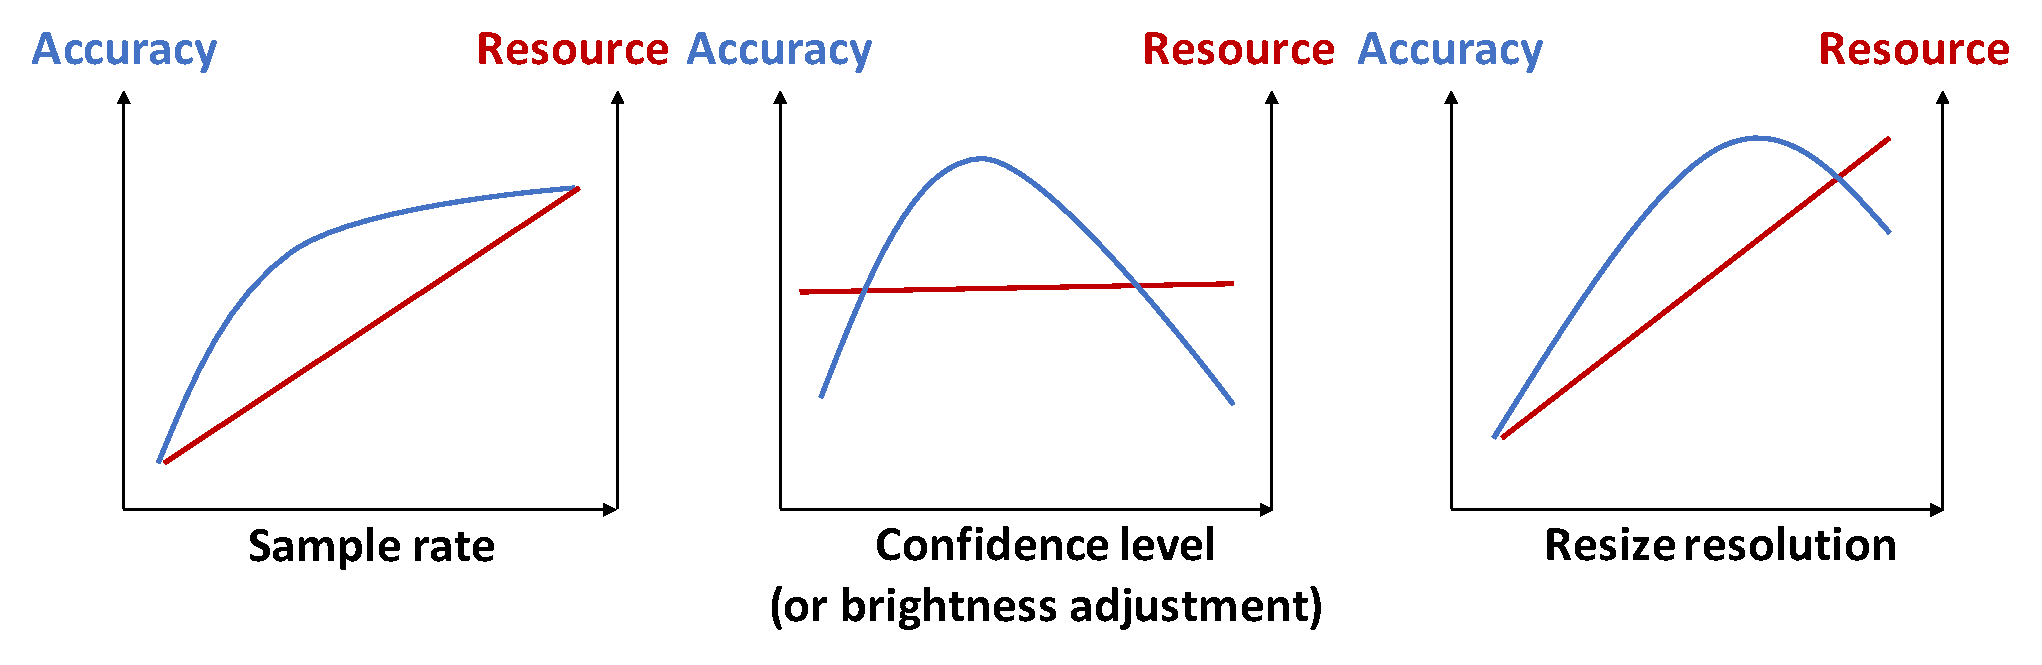
\includegraphics[width=0.52\textwidth]{figures/ImpactOfConfigs.pdf}
%\vspace{-0.2cm}
%\tightcaption{Impact of various configurations on the 
%resource-accuracy tradeoffs.}
%\label{fig:ImpactOfConfigs}
%\end{figure}

\begin{figure}[t!]
\captionsetup[subfigure]{justification=centering,farskip=-1pt,captionskip=5pt}
\centering
\hspace{-0.5cm}
\subfloat[Impact of frame sampling rate]
{
        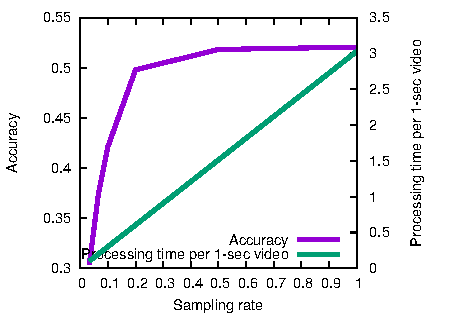
\includegraphics[width=0.35\textwidth]{PotentialFigures/ImpactAccuracy_Sampling.pdf}
        \label{fig:eval-overall-quality-jointime}
}
\hspace{-0.4cm}
\subfloat[Impact of input resolution]
{
        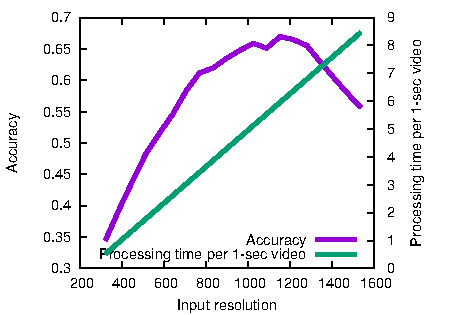
\includegraphics[width=0.35\textwidth]{PotentialFigures/ImpactAccuracy_Size.pdf}
        \label{fig:eval-overall-quality-jointime}
}
\hspace{-0.4cm}
\subfloat[Impact of confidence threshold]
{
        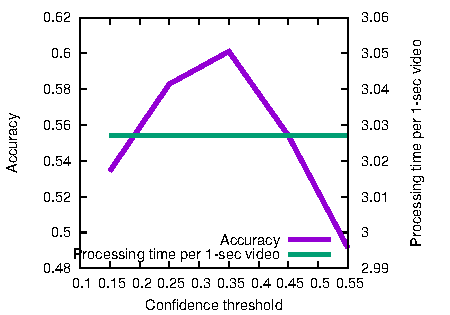
\includegraphics[width=0.35\textwidth]{PotentialFigures/ImpactAccuracy_Thresh.pdf}
        \label{fig:eval-overall-quality-jointime}
}
\hspace{-0.4cm}
\subfloat[Impact of frame brightness adjustment]
{
        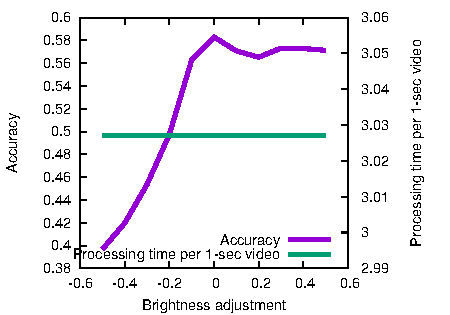
\includegraphics[width=0.35\textwidth]{PotentialFigures/ImpactAccuracy_Brightness.pdf}
        \label{fig:eval-overall-quality-jointime}
}
\hspace{-0.4cm}
\vspace{-0.2cm}
\tightcaption{Impact of various types of configurations on accuracy and resource consumption.}
%\vspace{-0.2cm}
\label{fig:eval-overall-quality}
\end{figure}

%\begin{packeditemize}

%\item 
\mypara{Changes in available resource}
First, when available resource increases, we can afford to run a more
expensive configuration (e.g., increase frame sample rate) to achieve
higher accuracy. 
Similarly, with less resource available, we need to run a cheaper 
configuration in order to keep real-timeness at the inevitable cost 
of relatively lower accuracy.
Figure~\ref{??} illustrates how optimal configurations vary in 
response to the changes of available resource.

%\item 
\mypara{Changes in resource-accuracy tradeoffs}
Second, if the resource-accuracy tradeoffs of configurations drift,
which can happen, as we show next, when video content changes,
the optimal configuration may change accordingly since the previous 
optimal configuration may yield a suboptimal resource-accuracy 
tradeoff now. 
Figure~\ref{??} illustrates how optimal configurations vary when 
resource-accuracy tradeoffs change due to dynamic video content.

%\end{packeditemize}

\begin{figure}[h!]
\centering
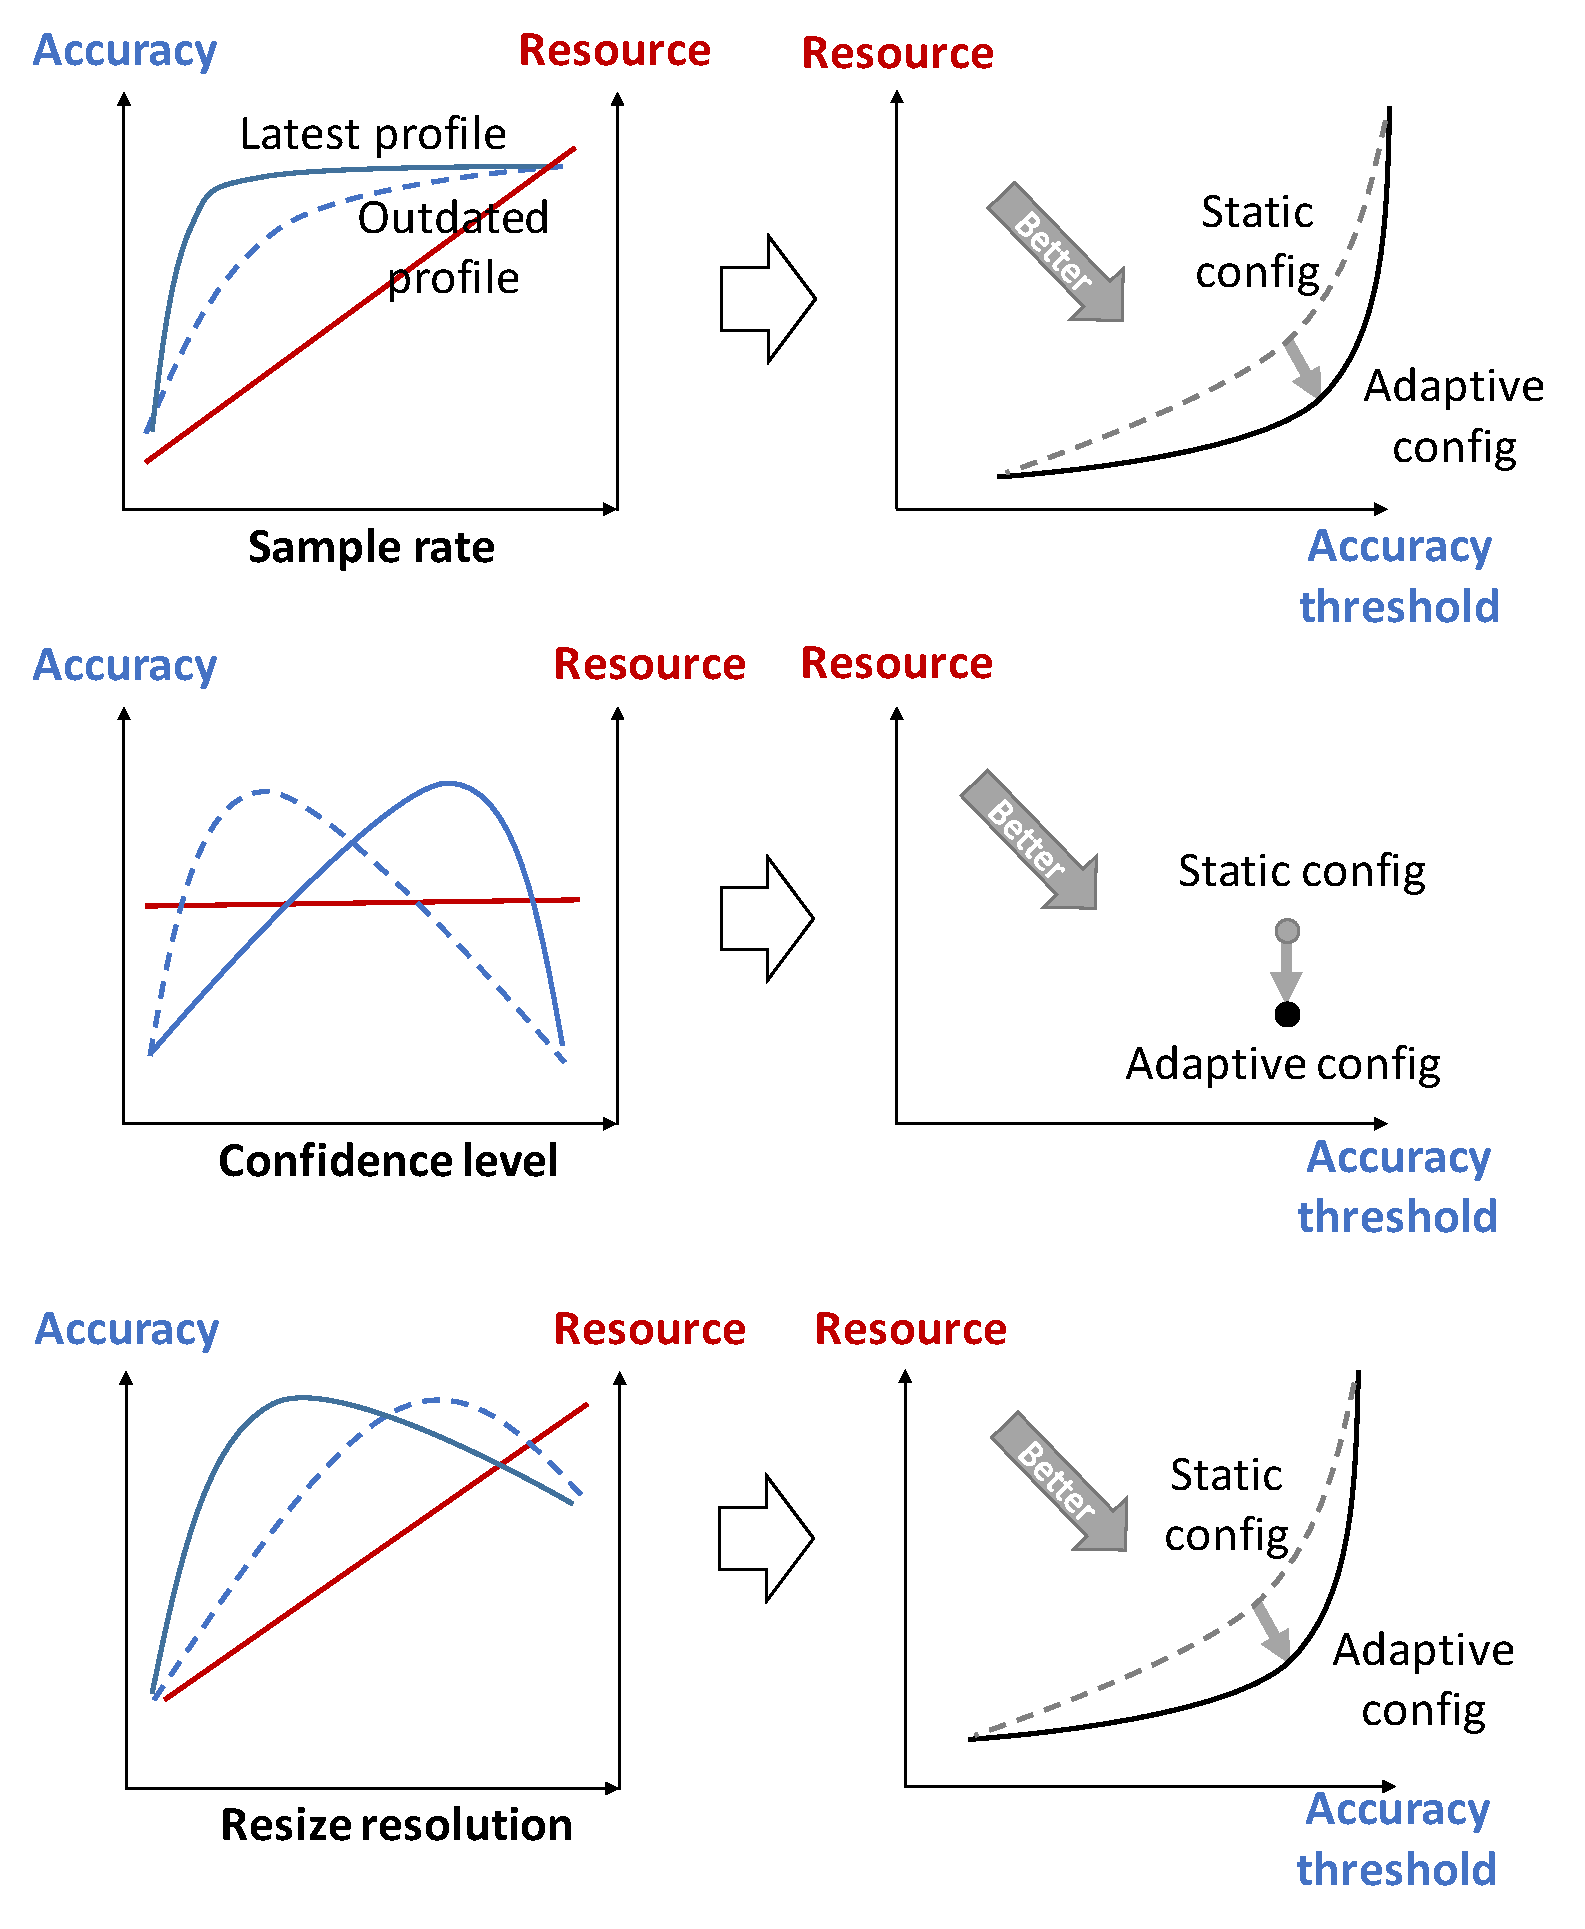
\includegraphics[width=0.45\textwidth]{figures/AdaptiveConfig.pdf}
\vspace{-0.2cm}
\tightcaption{How optimal configuration changes in response to 
dynamics profiles of resource-accuracy tradeoffs. 
Accordingly, assuming the static profiles will lead to suboptimal
performance.}
\label{fig:AdaptiveConfig}
\end{figure}

It is important to notice that these two sources of changes are 
orthogonal; that is, without any changes in available resource, the 
optimal configuration may change in response to drift in the profiles
of resource-accuracy tradeoffs.

%\mypara{Impact of video content on resource-accuracy tradeoffs}
Next, we take a closer look at what factors of video content can 
affect the resource-accuracy tradeoffs. 
Following are some factors that may change on the 
resource-accuracy tradeoffs of \nn:
\begin{packeditemize}
\item {\em Object velocity: }
\item {\em Video resolution: }
\item {\em Object size: }
\item {\em Bridghtness: }
\item {\em Confidence threshold: }
\end{packeditemize}


Moreover, optimal configurations are particularly prone to change 
during the cause of a query on live videos. 
This is because such query often
has long duration in which the video content is tend to vary in the 
aforementioned factors (e.g., car speed varies between peak and 
off-peak hours).

To summarize, the observations of dynamic configuration motivate the 
need for adapting configurations over time. 
